% These are some example steps 
% Refer https://www.overleaf.com/learn/how-to/Creating_a_document_in_Overleaf


\subsection{Sub Sections}

Use section and subsection commands to organize your document. \LaTeX{} handles all the formatting and numbering automatically. Use ref and label commands for cross-references.

\subsection{Comments}

Comments can be added to the margins of the document using the \todo{Here's a comment in the margin!} todo command, as shown in the example on the right. You can also add inline comments too:

\todo[inline, color=green!40]{This is an inline comment.}

\subsection{Tables and Figures}

Use the table and tabular commands for basic tables --- see Table~ \ref{tab:widgets}, for example. You can upload a figure (JPEG, PNG or PDF) using the files menu. To include it in your document, use the include graphics command as in the code for Figure~\ref{fig:Speed vs. Torque from Pittman} below.

\begin{table}[h]
\centering
\begin{tabular}{|l|r|}
\hline
Item & Quantity \\\hline
Widgets & 42 \\ \hline
Gadgets & 13 \\ \hline
\end{tabular}
\caption{\label{tab:widgets}An example table.}
\end{table}

% Commands to include a figure:
\begin{figure}[hbt!]
    \centering
    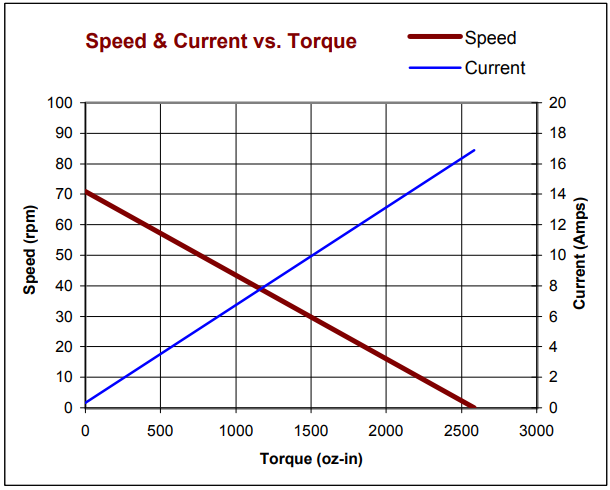
\includegraphics[width=0.9\textwidth]{Images/SpeedvsTorque.png}
    \caption{Speed vs. Torque from Pittman motor data sheet}
    \label{fig:Speed vs. Torque from Pittman}
\end{figure}





\subsection{Mathematics}

\LaTeX{} is great at typesetting mathematics. Let $X_1, X_2, \ldots, X_n$ be a sequence of independent and identically distributed random variables with $\text{E}[X_i] = \mu$ and $\text{Var}[X_i] = \sigma^2 < \infty$, and let
$$S_n = \frac{X_1 + X_2 + \cdots + X_n}{n}
      = \frac{1}{n}\sum_{i}^{n} X_i$$
denote their mean. Then as $n$ approaches infinity, the random variables $\sqrt{n}(S_n - \mu)$ converge in distribution to a normal $\mathcal{N}(0, \sigma^2)$.

\subsection{Lists}

You can make lists with automatic numbering \dots

\begin{enumerate}
\item Like this,
\item and like this.
\end{enumerate}
\dots or bullet points \dots
\begin{itemize}
\item Like this,
\item and like this.
\end{itemize}

%% cite an article
\subsection{Bibliography}
\begin{itemize}
    \item Adding bibliography to document
Some claim \cite{gratzer2007more}.
\end{itemize}

\subsection{Hyperlink to a website}
%% Hyperlink to a website
\begin{itemize}
    \item \href{https://www.overleaf.com/latex/templates/a-quick-guide-to-latex/fghqpfgnxggz}{Hyperlink to a website}.
\end{itemize}



\subsection{Learn LaTeX in 30 minutes}
\begin{itemize}
    \item \href{https://www.overleaf.com/learn/latex/Learn_LaTeX_in_30_minutes}{Link to overleaf website}.
\end{itemize}

